% Created 2025-03-29 Sat 12:35
% Intended LaTeX compiler: lualatex
\documentclass[11pt]{article}
\usepackage{fontspec}
\usepackage{graphicx}
\usepackage{lilyglyphs}
\usepackage{graphicx}
\usepackage{longtable}
\usepackage{wrapfig}
\usepackage{rotating}
\usepackage[normalem]{ulem}
\usepackage{amsmath}
\usepackage{amssymb}
\usepackage{capt-of}
\usepackage{hyperref}
\usepackage[cm]{fullpage}
\usepackage[headheight=15pt, headsep=10pt, top=1in, bottom=1in, left=0.75in, right=0.75in]{geometry} % Ensure sufficient header space
\setlength{\parindent}{0pt}
\usepackage{fancyhdr}
\pagestyle{fancy}
\fancyhf{}
\fancyhead[L]{\textbf{BV Scales For Jazz Improvization}} % Left header with title
\fancyhead[R]{\textbf{Bartev}} % Right header with author
\fancyfoot[C]{\thepage}
\fancyfoot[R]{Printed \today} % Right footer with today's date
\renewcommand{\headrulewidth}{0.4pt} % Optional: Add a horizontal rule below the header
\makeatletter
\let\ps@plain\ps@fancy % Apply "fancy" style to the first page
\let\maketitle\relax % Suppress default title/author rendering
\makeatother
\usepackage{multirow}  % Enables row spanning
\usepackage{array}     % Allows vertical centering
\usepackage{booktabs}  % Improves table aesthetics
\author{Bartev}
\date{2025-03-23}
\title{bv-scales-for-jazz-improv}
\hypersetup{
 pdfauthor={Bartev},
 pdftitle={bv-scales-for-jazz-improv},
 pdfkeywords={},
 pdfsubject={},
 pdfcreator={Emacs 29.4 (Org mode 9.6.15)}, 
 pdflang={English}}
\begin{document}

\maketitle

\section{Common scales for major, dominant and minor chords}
\label{sec:org94af96e}

\begin{center}
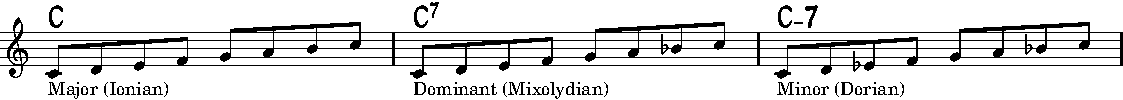
\includegraphics[width=.98\linewidth]{maj-myx-dor.pdf}
\end{center}

\section{Scales for half diminished chords}
\label{sec:org5fd82fd}
\subsection{Locrian}
\label{sec:org40261c9}
Play the scale 1/2 step higher (D\flat) starting on the 7th (C)
\begin{center}
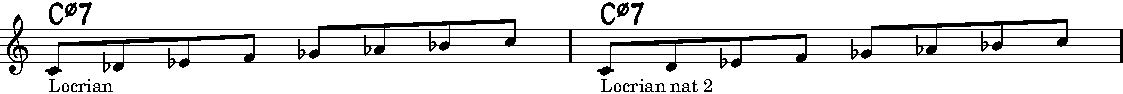
\includegraphics[width=.98\linewidth]{half-dim-chords.pdf}
\end{center}

\subsection{Two ways of looking at the half/whole (H/W) diminished scale.}
\label{sec:org3fd8170}

It contains the chord tones for a half diminished chord. (\flat3, \flat5, \flat7)

It can work for chords like C7(\sharp9), C7(\flat9), C7(13\flat9) = C7(13) = (C7\sharp5)

\begin{center}
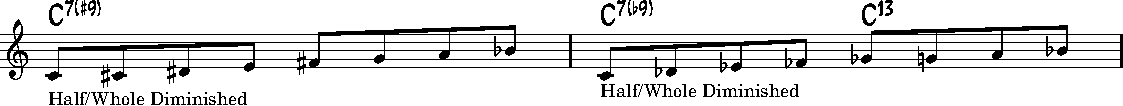
\includegraphics[width=.98\linewidth]{half-whole-dim.pdf}
\end{center}

This is the same scale starting on any of the 4 notes C, E\flat, F\sharp, or A.

There are only 3 distinct H/W scales.

\begin{center}
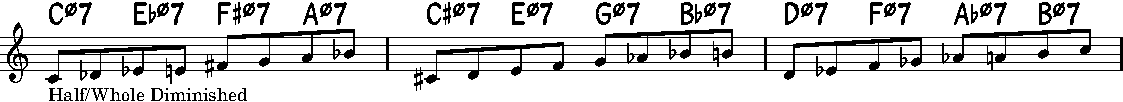
\includegraphics[width=.98\linewidth]{half-whole-dim-3.pdf}
\end{center}

\subsection{Altered Scale}
\label{sec:orgcd74133}
Three ways of looking at the altered scale.

It is very similar to the half/whole diminished.

You can also look at it as having the notes of the scale a 1/2 step lower.
\begin{center}
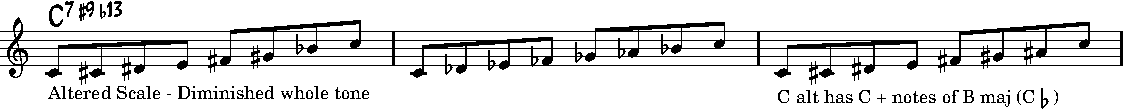
\includegraphics[width=.98\linewidth]{altered.pdf}
\end{center}

Another way of thinking of it is as the notes of the melodic minor (\flat3) starting 1/2 step up.

\begin{center}
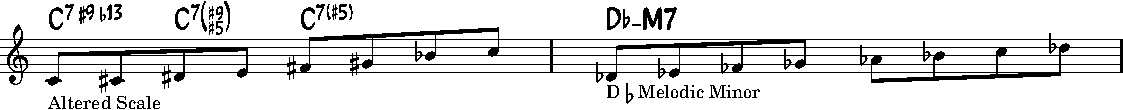
\includegraphics[width=.98\linewidth]{altered-as-melodic-minor.pdf}
\end{center}

\section{Diminished chords (W/H Dim)}
\label{sec:org8104e4a}
Two ways of looking at the whole/half diminished.

You can think of this as a diminished chord (C, E\flat, G\flat, B\flat\flat) plus a whole step above each chord tone (D, F, A\flat, C\flat).

\begin{center}
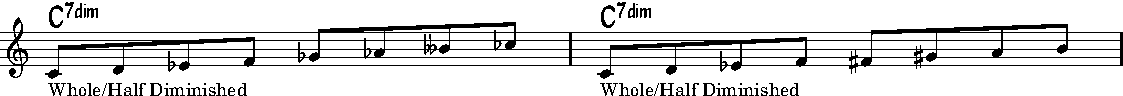
\includegraphics[width=.98\linewidth]{whole-half-dim.pdf}
\end{center}

There are only 3 distinct W/H scales.

\begin{center}
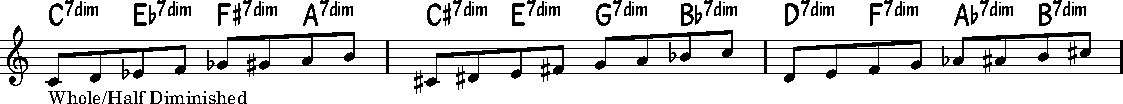
\includegraphics[width=.98\linewidth]{whole-half-dim-3.pdf}
\end{center}

\section{Lydian Chords}
\label{sec:orgd6df5f5}
The Lydian scale has a raised 4th (11th). (4th mode of major scale)

Dominant indicates a lowered 7th.

Augmented indicates a raised 5th.
\begin{center}
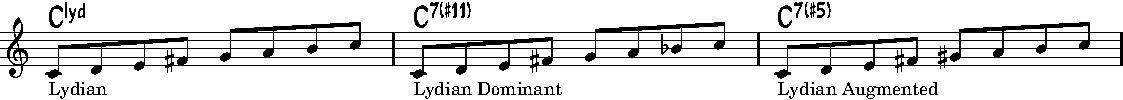
\includegraphics[width=.98\linewidth]{lydian.pdf}
\end{center}

\section{Phrygian (Spanish) Dominant}
\label{sec:org578086f}

The Phrygian (Spanish) dominant scale is the 5th mode of the Harmonic minor scale (\flat3, \flat6).

It has an exotic sound.
\begin{center}
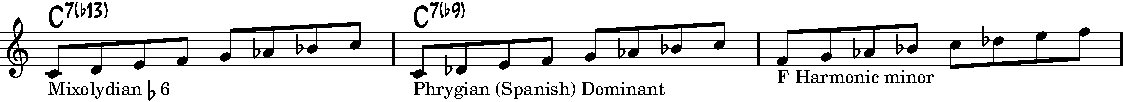
\includegraphics[width=.98\linewidth]{phrygian.pdf}
\end{center}

\section{Whole tone}
\label{sec:org0f918f8}

There are only 2 whole tone scales. (Both given below.)
\begin{center}
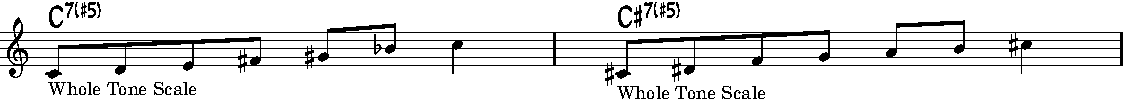
\includegraphics[width=.98\linewidth]{whole-tone.pdf}
\end{center}

\section{Minor Scales}
\label{sec:org6058482}
Natural Minor: Add 3 \flat's (\flat3, \flat6, \flat7)

Harmonic Minor: \flat3 \& \flat6 (natural minor with raised [natural] 7)

Melodic minor: \flat 3 - Classical music has melodic minor rising, and natural descending.

\begin{center}
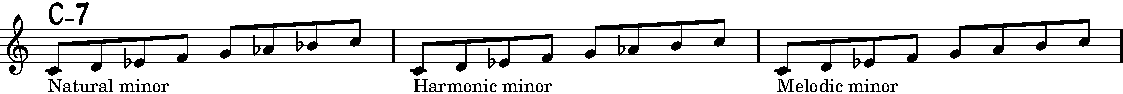
\includegraphics[width=.98\linewidth]{minor-scales.pdf}
\end{center}

\section{Pentatonic and Blues}
\label{sec:org9c66ef4}

The minor pentatonic has the same notes as the major pentatonic of the relative minor.

C minor pentatonic has same notes as the E\flat  major pentatonic.

The blues scale is like the minor pentatonic with an added "blues" tone (\sharp4)

\begin{center}
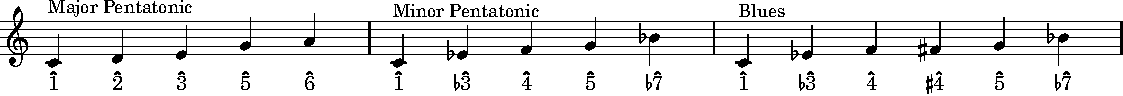
\includegraphics[width=.98\linewidth]{pent-blues.pdf}
\end{center}

\section{Chord Choices}
\label{sec:org618a9b1}

\begin{center}
\begin{tabular}{lllll}
Chord & Basic &  &  & More altered\\[0pt]
\hline
maj7 & Ionian & Lydian & Lydian \sharp5 & \\[0pt]
min7 & Dorian & Aeolian & Phrygian & \\[0pt]
dom7 & Mixolydian & Lydian \flat7 & \flat9 diminished & altered\\[0pt]
half-dim (min7 \flat5) & Locrian & Locrian nat9 &  & \\[0pt]
minMaj7 & Melodic minor &  &  & \\[0pt]
Maj7 \sharp5 & Lydian \sharp5 &  &  & \\[0pt]
dom7 \sharp11 & Lydian \flat7 &  &  & \\[0pt]
dom7 \flat9 & Altered &  &  & \\[0pt]
dom7 \sharp8 \flat13 & Altered &  &  & \\[0pt]
altered dom & Altered &  &  & \\[0pt]
\end{tabular}
\end{center}

\section{Modes of scales}
\label{sec:orgb792a21}

\begin{table}[h]
\centering
\begin{tabular}{|c|c|c|}
\hline
Mode & Major & Melodic Minor \\
\hline

\multirow{4}{*}{\centering \textbf{1}} & Ionian &  \\
& Major & Minor  \\
&  & \flat 3 \\
&  & Use over minMaj7 \\
\hline

\multirow{3}{*}{\centering \textbf{2}} & Dorian &  Dorian \flat 2\\
&  Minor &  Minor \\
& \flat 3, \flat 7 & \flat 2, \flat 3, \flat 7 \\
\hline

\multirow{5}{*}{\centering \textbf{3}} & Phrygian &  Lydian \sharp5 \\
&  Darker minor &  Major \\
& Add 4 \flat's & \sharp4, \sharp5 \\
&  & Use over Maj7 \sharp5 \\
&  Not the same as Phrygian dom &  \\
\hline

\multirow{5}{*}{\centering \textbf{4}} & Lydian &  Lydian \flat7 \\
&  Major & Major \\
& Add 1 \sharp &  \sharp4, \flat7\\
&  & Use over dom \sharp11 \\
&  Not the same as Phrygian dom &  \\
\hline

\multirow{4}{*}{\centering \textbf{5}} & Mixolydian & Mixolydian \flat6 \\
&  Major & Major \\
& Add 1 \flat &  \flat6, \flat7\\
&  Use over dom 7 &  \\
\hline

\multirow{5}{*}{\centering \textbf{6}} & Aeolian & Locrian nat9 \\
&  Natural minor &  \\
&  \flat3, \flat6, \flat7 &  lower 5th, raise 9th \\
& Add 3 \flat's &  \\
&  & Use over half-dim (min7 \flat5)  \\
\hline

\multirow{8}{*}{\centering \textbf{7}} & Locrian & Altered \\
&  Half-diminished &  \\
&  \flat2, \flat3, \flat5, \flat6, & \\
& Add 5 \flat's &  \\
&  Use over half-dim (min7 \flat5) & Use over altered dom  \\
&  & Use over dom7 \flat9  \\
&  & Use over dom7 \sharp9 \flat13  \\
& Key of scale 1/2 step higher than root & \\
\hline

\end{tabular}
\caption{Modes of Scales}
\end{table}
\end{document}
